\chapter{\Cref{part:glenside-and-3la} Introduction and Motivation}
\label{sec:part1-motivation}

\hl{copied from glenside intro}
Machine learning (ML) and other
  high-performance computing (HPC)
  applications increasingly rely on
  specialized hardware accelerators to
  provide speed and energy efficiency~\cite{jouppi2017tpu, krizhevsky2012conv, reuther2019survey}.
This trend has highlighted the need
  for flexible accelerator support
  in domain-specific compilers like
  Halide~\cite{halide},
  TVM~\cite{chen2018tvm},
  TensorFlow/MLIR~\cite{tensorflow, mlir}, and
  PyTorch~\cite{pytorch}.

Adding accelerator support to
  an existing compiler typically
  uses custom pattern matching to
  map expensive tensor operations
  from applications down to
  accelerator invocations~\cite{
    yang2020interstellar, byoc}.
Pattern matching often additionally relies on
  various other transformations
  to canonicalize intermediate representations (IRs)
  %~\cite{??}
  and massage data layouts into
  formats matching accelerator requirements~\cite{nvidia2020nhwc}.
Even with these changes,
  users may need to manually modify their application to
  help the compiler discover opportunities
  for dispatching operations to accelerators, 
  such as by changing data types or unrolling loops.
\hl{end copied from glenside intro}

% Top-level points: 
% We need something like the 3LA methodology;
% 3LA methodology needs flexible matching.


% WE NEED SOMETHING LIKE 3LA METHODOLOGY
% Points:
%% Hardware acceleration is important.
%% Accelerators are nothing without testing/without compilers? which one?
%% Need a methodology for building compilers.

%% Hardware acceleration is important.

Hardware acceleration has powered significant advances
  in subfields like artificial intelligence, image processing, and graph analysis~\cite{han2016eie,chen2016eyeriss,reagen2016minerva,zhang2016cambricon,hameed2010understanding,ham2016graphicionado,jouppi2017tpu, krizhevsky2012conv, reuther2019survey}.
This trend has highlighted the need
  for flexible accelerator support
  in domain-specific compilers like
  Halide~\cite{halide},
  TVM~\cite{chen2018tvm},
  TensorFlow/MLIR~\cite{tensorflow, mlir}, and
  PyTorch~\cite{pytorch}.

Despite our increasing dependence
  on accelerators,
  building compilers
  for custom accelerators
  remains a daunting task.
Paralleling the thesis of this dissertation,
  we will describe the challenges
  of building compilers
  along three axes:
  \cref{thesis:devtime},
  \cref{thesis:optimizations},
  and \cref{thesis:correctness}.
  

\paragraph{
\cref{thesis:devtime}.
}
Current frameworks for compiler generation
  generally require significant compilers expertise,
  and the sheer amount of effort
  required to build a compiler from the ground up
  generally limits bespoke compiler construction
  to teams
  at large companies,
  e.g. the TensorFlow 
  stack~\cite{abadi2016tensorflow}
  for Google's 
  TPU~\cite{jouppi2017tpu,jouppi2020tpu}.
Though projects
  such as 
  MLIR~\cite{mlir,
  lattner2021mlir,
  eldridge2021mlir}
  and
  Exo~\cite{ExoPldi22}
  have begun to prescribe
  a general framework
  for structuring a compiler,
  these tools are built for
  domain experts,
  and require significant time investment
  \hl{vague}.
There is a need for
  automated techniques
  for compiler generation,
  to lower the barrier
  and allow non-experts to generate
  functioning compilers.
An example of such a technique
  is the deep learning compiler
  TVM's~\cite{chen2018tvm}
  Bring Your Own Codegen (BYOC)
  framework~\cite{chen2021byoc}.
\hl{tease at how BYOC will fail? or handle in optimizations?}
Though, 
  as we will show later,
  while BYOC makes it easy for
  users to add basic support
  for accelerators,
  we will see 
  that its ability to 
  match workloads to accelerators
  is lacking.

\paragraph{
\cref{thesis:optimizations}.
}
Even once a compiler is constructed,
  they still have the tendency
  to leave optimizations on the table---%
  especially user-facing compiler construction frameworks.
\hl{As a consequence, optimizations can be left on the table.
Note that simply mapping to accelerators
  is considered an optimization,
  but e.g.~mappings can be missed.}
Even once a compiler
  is constructed
  for a piece of custom hardware,
  it can still leave optimizations
  on the table.
Getting a compiler to realize
  that a certain operator
  can be run on an accelerator,
  for example,
  may require syntactic changes
  to the input program,
  especially when using
  a matcher like
  BYOC.

% And the difficulties
%   in building a quality compiler
%   often lead hardware designers to forego the process
%   entirely, which can
%   hinder or entirely prevent
%   the validation and testing
%   of custom hardware,
%   leading to expensive bugs
%   (\cref{thesis:correctness}).

\paragraph{
\cref{thesis:correctness}.
}
Core to developing
  accelerators
  quickly and correctly
  is the process of \textit{hardware validation.}
\hl{glossary terms: validation, testing, verification}
\textit{Validation}
  of hardware---%
  the process of testing
  whether the hardware behaves
  how the designer intended---%
  is important.
An immense amount of effort
  and money
  is currently put
  into hardware validation and testing.
\hl{how much is spent on hw validation compared to sw}  
Despite the growing dependence
  on accelerators,
  testing custom hardware is still largely
  a manual, ad hoc, and difficult process.
A primary challenge in 
  accelerator development
  is validating designs
  on real applications.
This validation
  is critical,
  as some accelerator bugs 
  arise
  only during validation
  of full applications.
For example,
  a deep learning
  accelerator may use
  a custom numeric format
  tuned to be storage-efficient,
  while still providing enough
  precision
  to support effective inference.
Testing the numeric format
  on a single layer
  of the deep learning model
  may produce results
  well within the designer's
  error bounds.
However, if the designer
  neglects to test
  \textit{all}
  layers of the model,
  they may fail to discover that,
  even though individual layers
  behave well,
  the error may accumulate
  across layers,
  producing inaccurate application-level results~\cite{zorn2021rounding}.
Early end-to-end application level validation is thus essential
  for avoiding expensive and complex late stage hardware design changes.
\hl{merge or delete below}
In general,
  thorough validation
  is inaccessible
  to the common designer.
The most intensive validation
  is done in industry,
  where companies can hire full-time
  engineers
  to do validation
  on designs.
\hl{reference fig} \cref{fig:3la-pie}

\begin{figure}
\centering
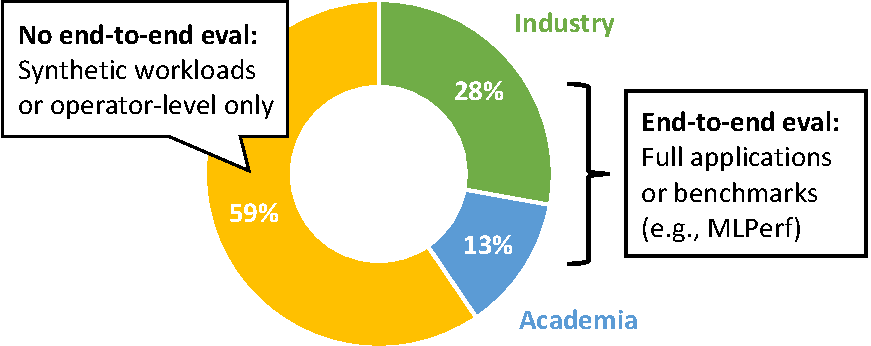
\includegraphics[width=.6\textwidth]{assets/3la-pie.pdf}
\caption{
\hl{this figure is taken from ...cite 3LA...update caption}
\textbf{Gap in end-to-end evaluation of accelerators for neural network applications:} 
Survey of papers from ISCA, MICRO, VLSI, and ISSCC in 2021 and ICCAD, DAC in 2020.
Our survey of $79$ papers  that introduced new DL accelerator designs/methodologies, comparing how the accelerators were evaluated. Only 41\% of the works reported end-to-end evaluation on non-synthetic applications, of which 68\% (28\% of the total) were from industrial teams.
}
\label{fig:3la-pie}
\end{figure}


  
When validation \textit{is} done
  outside of industry,
  it is often not done end-to-end.
Not only is it important
  to test \textit{components}
  of a hardware design;
  it is also important
  to test full applications end-to-end.
Hardware specialization and customization often
  requires changing memory hierarchies,
  data representations~\cite{chan2014itrs,fang2019understanding,lai2021programming}.
Issues arising from these complex
  microarchitectural changes
  may not manifest
  at the component level---%
  for example, a reduced-bitwidth
  ALU
  may still produce accurate results,
  but overall \textit{application}
  performance
  may suffer
  due to the change in numeric behaviors.
\hl{call forward to evaluation}
Testing is often 
  too commonly poorly done.
\hl{insert figure from 3LA}

%% Need a methodology for building compilers.

In response to the challenges
  of hardware validation
  to the common designer,
  Huang et.~al.~developed
  3LA:
  a methodology
  to make testing
  easier for new accelerator designs~\cite{huang2022specialized,huang2024application}.
The primary contribution of 3LA
  is 
  a methodology to end-to-end evaluate accelerators on unmodified, full applications.
\hl{fix 3LA citation: i think it might be duplicated, and update it todaes.}
\hl{Explain how we're just a component of 3LA.}

\begin{figure}
    \centering
    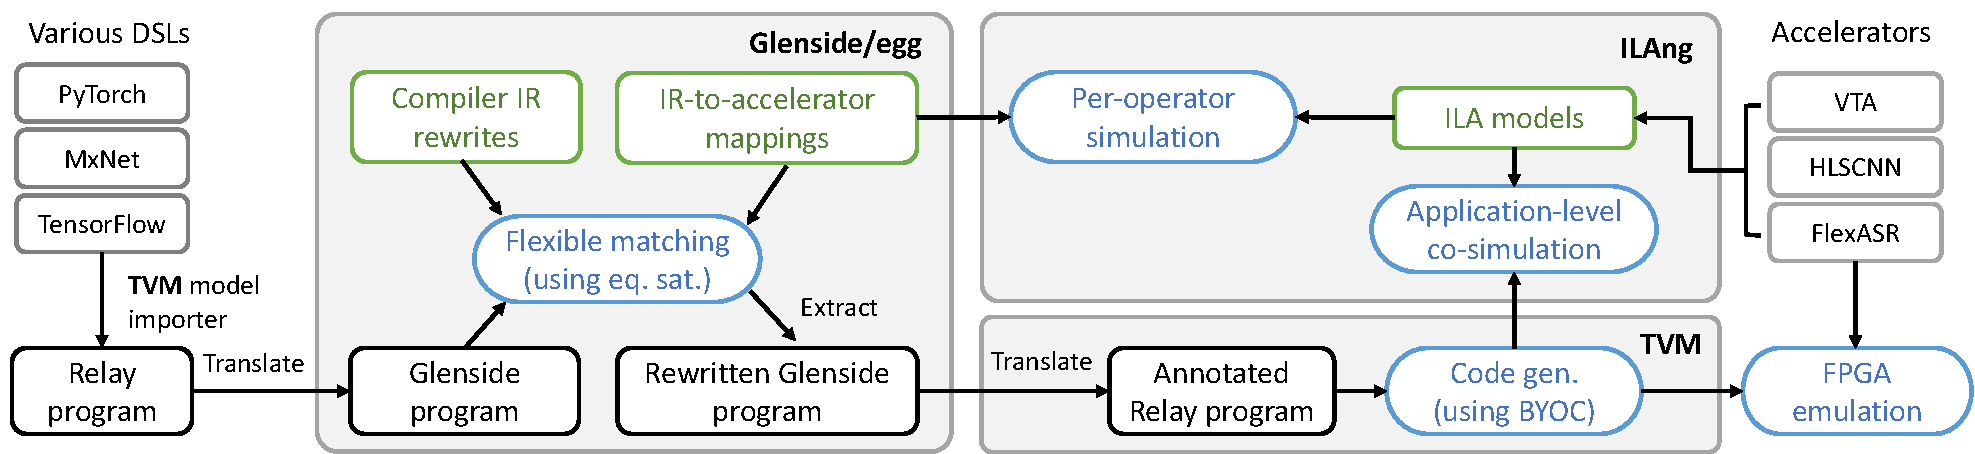
\includegraphics[width=\textwidth]{assets/3la-diagram.pdf}
    \caption{
    \hl{not quite sure where this goes}
This figure first appeared
  in Huang et.~al.~\cite{huang2024application}.
Diagram of the 3LA prototype's flow.
Note that only the ``Glenside/egg''
  portion of 3LA
  is considered a contribution
  of this dissertation;
  for more information on the other components,
  please see the original paper.
}
    \label{fig:3la-diagram}
\end{figure}

3LA solves two major problems:
  first, generating simulators
  for hardware
  is difficult
  and time consuming.
Second, even given a simulator
  for your design,
  it is then difficult
  to run full applications
  on the simulator.
  
3LA solves the first problem
  using the Instruction-Level Abstraction (ILA)~\cite{huang2018instruction,huang2018formal}.
ILA is a specification system
  originally designed for
  system-on-chip verification purposes.
The authors of 3LA
  repurposed the ILA
  as a tool for capturing
  and simulating
  machine learning accelerator behavior,
  giving accelerator developers
  a framework for generating fast,
  high-level simulators
  for their accelerators.
The first contribution
  of 3LA
  we do not consider
  a contribution of this dissertation;
  please refer to the dissertation
  of Bo-Yuan Huang~\cite{huang2022instruction}
  and Steven Lyubomirsky~\cite{lyubomirsky2022compiler}
  for more information about 3LA as a whole.

However,
  the second challenge of 3LA:
  namely that, even given a simulator,
  running full programs on your simulator
  is difficult,
  is much more pertinent.
Specifically, the challenge
  is that
  compiling to custom hardware
  (whether real or simulated) is difficult,
  and, at the time of developing 3LA,
  there were few open-source, flexible 
  compiler frameworks
  for targeting custom hardware.

One open-source framework
  supporting mapping
  to custom accelerators
  is TVM's Bring Your Own Codegen (BYOC)~\cite{byoc,chen2021byoc}.
Initially, the 3LA authors
  attempted to use BYOC
  to address their second issue.
To use BYOC, the user
  provides syntactic patterns
  which BYOC then searches for
  in the workloads of interest.
However,
  exact syntactic pattern matching 
  (which we refer to simply as
    ``exact matching'')
  faces difficulties
  as there is often no canonical way
  to represent an operation,
  necessitating either the addition of more patterns
  or manual modifications to the input program
  to match the expected patterns.
Application code can vary greatly in structure,
  particularly in the case of compiler IRs,
  which may be produced after several iterations
  of program transformations.
Code variations are especially prevalent
  in machine learning compilers,
  where workloads are often imported
  from other languages via importers.
Even for the same machine learning model,
  importers from different languages
  can produce wildly different (but equivalent)
  imported programs.
 
This is where I was able
  apply my dissertation.
We developed a language
  called \g
  which allowed for the application
  of equality saturation


%% GLENSIDE INTRO

\hl{I would summarize the glenside intro here, and then provide the full intro in the glenside chapter.}
Adding accelerator support to
  an existing compiler typically
  uses custom pattern matching to
  map expensive tensor operations
  from applications down to
  accelerator invocations~\cite{
    yang2020interstellar, byoc}.
Pattern matching often additionally relies on
  various other transformations
  to canonicalize intermediate representations (IRs)
  %~\cite{??}
  and massage data layouts into
  formats matching accelerator requirements~\cite{nvidia2020nhwc}.
Even with these changes,
  users may need to manually modify their application to
  help the compiler discover opportunities
  for dispatching operations to accelerators, 
  such as by changing data types or unrolling loops.
\hl{
These modifications may be especially
  untenable
  for hardware developers,
  who may not have practical experience
  with the workloads
  and toolchains. 
(something tying it in to new combined intro)
}
    
In principle, term rewriting techniques~\cite{baader1998term}
  should be able to facilitate many of
  these transformation and mapping tasks
  within a compiler.
Halide and TVM already rely
  on extensive rewrite systems for
  optimizing scalar computations and
  simplifying loop bounds in order to
  support further downstream optimizations~\cite{newcomb2020halide-rewrite,
  hagedorn2020func-high-perf}.

Unfortunately, existing IRs in compilers for
  array/tensor programming DSLs tend to
  present abstraction and granularity mismatches
  that hamper term rewriting approaches.
Term rewriting is most easily applied in
  \textit{pure} (side effect--free) IRs
  that support equational reasoning.
At the same time,
  mapping to accelerators requires considering
  low-level hardware details like data layout.
Existing pure IRs for ML frameworks are used
  primarily for high-level transformations
  (e.g., type elaboration and inlining)
  and do not expose low-level data layout details~\cite{relay}.
On the other hand,
  IRs used for crucial lower-level optimizations like
  operator fusion must support
  precise reasoning about memory use,
  and therefore are typically impure,
  hampering term rewriting.% approaches.

To help mitigate such impedance mismatches,
  we present \textit{\g},\footnote{Publicly available at \url{https://github.com/gussmith23/glenside}.}
  a pure tensor program IR
  that enables hardware-level term rewriting.
\g is based on a simple
  \textit{access pattern} abstraction that
  supports expressing and reasoning about
  data layout transformations via
  syntactic rewrite rules.
  \begin{figure}
    \centering
    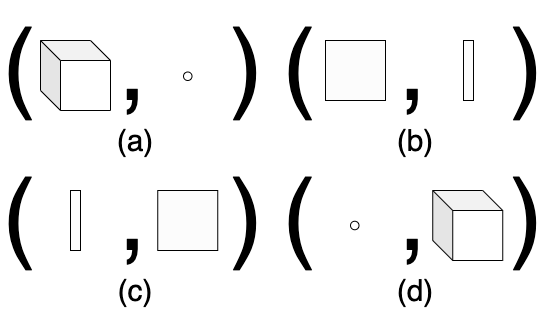
\includegraphics[width=.6\linewidth]{glenside/access-pattern-examples-2x2.png}
    \caption{
      Four access patterns,
        representing different ways
        a
        tensor program
        (or \textit{kernel})
        might access
        the same 3D tensor. 
      For example, (c) represents
        accessing a 3D tensor as
        a vector of 2D matrices.}
    \label{fig:access-pattern-examples}
    \vspace{-1em}
\end{figure}
When combined with standard arithmetic rewrites
  for per-tensor-element computations,
  access patterns enable implementing complex
  transformations for accelerator support as
  compositions of simple rewrites.

Tensors are traditionally characterized
  by their \textit{shape},
  an $n$-tuple 
  %in $\mathbb{N}^n$
  of positive integers
  indicating the size of each
  of a tensor's dimensions.
  % , e.g., $(x, y, z)$ for a 3D tensor.
Access patterns instead characterize
  each tensor with two shapes, e.g.,
  \accesspatternshape{x}{y, z}, separating
  the dimensions which are \textit{iterated over} from
  the dimensions which are \textit{computed on.}
Figure~\ref{fig:access-pattern-examples}(c)
  depicts an example where a 3D tensor's
  first dimension is iterated over and
  some computation applied to each
  corresponding 2D matrix.

\g \hl{
 plays a crucial role in the 3LA framework.
}
We demonstrate how \g
  enables implementing representative
  hardware-level transformation via term rewriting,
  including mapping computations
  to systolic arrays~\cite{jouppi2017tpu}
  (a common hardware module in ML accelerators)
  and automatically discovering the
  \tcd{im2col} data layout transformation~\cite{im2col},
  which enables mapping 2D convolutions
  to matrix multiplication hardware.
In particular,
  by employing \textit{equality saturation}~\cite{willsey2021egg},
  these transformations ``fall out for free''
  (i.e., without any carefully crafted
  rewrite orderings~\cite{phase-ordering}),
  from a handful of general rewrites concerning tensor
  transposition, Cartesian product, dot product, etc.,
  expressed in terms of access patterns.


\hl{move this to glenside chapter?}
 The rest of this chapter is organized as follows:
Section~\hl{todo} provides background
  and briefly surveys closely related work.
Section~\ref{sec:matmul} motivates
  \g via a running example exploring
  pure matrix multiplication.
Section~\ref{sec:glenside} details the
  design and implementation of \g.

%% END GLENSIDE INTRO

Skipping over the comparisons with related work.
If we include anything, it should be something
  from the Task 1 paraagraph, re comparison with Exo, MLIR, etc.

Should take something from "detailed comparison
  with closely related tools".

Background. Can probably skip 2.1.

Probably want 2.2. But maybe should just be the Glenside chapter.

But then we need to find a way
  to lead into the Glenside intro.

Would be great to set up this chapter
  so that it ends with a very clear statement
  of what we need our language to do.
Then the Glenside chapter can do those things.
But we also need to make sure
  we tie it back to the thesis.


  To summarize, the contributions of this chapter include:
\begin{itemize}
\item \textit{Access patterns},
  a tensor representation that employs a
  simple, extended tensor shape type to
  distinguish iteration and computation dimensions

\item The \g IR,
  a pure compiler IR that facilitates 
  term rewriting to enable support for
  specialized accelerators
  
\item A library of generic rewrites over \g programs
  
% \item Case studies demonstrating how
%   \g enables automatically discovering
%   key transformations for mapping
%   applications to custom accelerators
%   via equality saturation with the
%   \tcd{egg}~\cite{willsey2021egg} library.
\end{itemize}


% 3LA methodology needs flexible matching.
\section{Summary of the 3LA Methodology}

The 3LA methodology as a whole
  (or just 3LA for short)
  is not a contribution of this dissertation---%
  see the dissertations of
  Bo-Yuan Huang~\cite{huang2022instruction}
  and 
  Steven Lyubomirsky%
  ~\cite{lyubomirsky2022compiler}.
However,
  \g, a contribution of this dissertation,
  is a 
  significant component of 3LA,
  and its development 
  is inextricably linked to the development
  of 3LA.
As such,
  some understanding of the 3LA
  methodology
  is required for understanding
  \g.
  


\hl{
Copied from 3LA paper, rephrase: 
}

The ILA is an ISA-like formal model 
  for specifying the functional behavior of accelerators.
It generalizes the ISA to accelerators, 
%and provides a modular functional specification as a set of instructions. Each 
  where each 
  instruction of an accelerator ILA corresponds 
  to a command at the accelerator interface, i.e., an MMIO load or store from a host processor.
Like processor ISAs, 
  the ILA captures a formal semantics of the accelerator behavior, by specifying how each instruction 
  reads or updates software-visible (viz., architectural) state variables in the accelerator,
  while abstracting out implementation details. 
  
Fig.~\ref{fig.ila-example} shows an example
  ILA specification for one of the instructions of FlexASR~\cite{tambe20219} (one of the three accelerators used in our evaluation studies). The ILA models are written in ILAng, a DSL embedded in C++. The figure caption points out the per-instruction modular specification, where each instruction is specified by defining its decode condition (i.e., when the instruction is triggered) and state update functions (i.e., how it updates
  the architectural state variables). 
  %updates are specified.

Thus far, the ILA has been used only for accelerator implementation verification and co-verification of firmware~\cite{huang2018formal,huang2018instruction}.
In this work, we use ILA as a formal SW/HW interface that drives the key tasks in compilation and application-level testing for accelerators.

\hl{end copy from 3LA }